%%% File encoding is ISO-8859-1 (also known as Latin-1)
%%% You can use special characters just like �,� and �

\chapter{Background}

\section{Consensus Mechanism and Proof-of-Stake}
In a fiat currency, there is a central body that makes decisions in regards to which transactions are valid and which order the transactions should be processed in. However, for decentralized currencies, there is no single decision maker. The method through which cryptocurrencies make decisions is through consensus. For a public ledger of transactions, such as Bitcoin and Ethereum, there must exist a method for the participants of the network to come to a consensus on which transactions should be added to the ledger. In the most general sense, consensus works by temporarily granting authority to one or more nodes, allowing them to choose a block of transactions that get processed. Then, the rest of the nodes in the network can either accept that block or reject it. If a majority of the network accepts it, then that block gets added to the ledger.

There are many different protocols for a network to come to a consensus. The most popular protocol is Proof of Work, which involves having each node perform computationally heavy work and submit proof. It is usually done in the form of solving a hash puzzle. In a hash puzzle, every node has to try to generate a hash from a random input, such that it can fulfill a set condition. Among competing miners, the node that solves the puzzle first is awarded the authority to create the new block of transactions. In the second most popular protocol, Proof-of-Stake, every node locks up a certain amount of their own wealth as a collateral. Then out of these nodes, one or more are algorithmically chosen to determine the next block. The original principle of Proof-of-Stake, where nodes who stake more are given a larger reward, can worsen the centralization problem. As a result, variations, such as Pure Proof-of-Stake, Delegated Proof-of-Stake, and Extended Proof-of-Stake, have been developed.

\section{Metrics for Measuring Centralization and Inequalities in Crypto-currencies}
Going further, as we developed a system to reduce centralization in cryptocurrencies, we needed a method to measure centralization in order to verify if our solution was effective. In terms of wealth, there are a few available metrics to measure centralization: percentage value, the Theil index, and the Gini coefficient. The simplest and most intuitive measurement is through percentage value. Percentage value is the percentage of total wealth the richest X amount of nodes hold. So a common measurement in economics is to find what percentage of wealth the top 1\% of a country holds. For example, in 2017, the US Federal Reserve reported that the top 1\% richest Americans held around 38.5\% of the nation's total wealth. However, we can get more accurate estimates of wealth centralization. The Theil index is used in socio-economics as a measurement of entropy across a population. It is commonly used to measure income inequality and racial segregation. It can be mathematically represented by the equation \cite{CRYPTO:7}
\begin{equation} 
T_{T} = \frac{1}{N}\sum_{i=1}^{N}\frac{x_{i}}{\mu}\ln\left ( \frac{x_{i}}{\mu} \right ) \end{equation}
where $x_{i}$ is the income of person $i$ and $\mu$ is the mean income:
\begin{equation} 
\mu = \frac{1}{N}\sum_{i=1}^{N}x_{i}
\end{equation}
If everyone has equal income, $T_{T} = 0$. If one person holds all the money, then $T_{T} = \ln(N)$.

While the Theil index will give us a fairly accurate measure of centralized wealth, we want to create a comparison across different kinds of Proof-of-Stake systems implemented in our simulations. So we need our measurement to be standardized, which is why we are going to be using the Gini coefficient. It is used generally as a measure of statistical dispersion in a given population; more specifically, it measures inequality among frequency distributions, which is why it is used to measure wealth inequality. The Gini coefficient is represented by a percentage ratio whereby 0 means a perfectly equal distribution, and 1 represents one person holding all the wealth. Global powerhouses like the US, China, France, and Germany have their Gini coefficient between 31-44\%, while cryptocurrencies like Bitcoin and Ethereum have a coefficient at 99\%. Mathematically speaking, the Gini coefficient is derived from the Lorenz curve which is a graphical representation of wealth distribution, mapping population on the X-axis and wealth percentage on the Y-axis \cite{CRYPTO:6}.
\begin{figure}[H]
\begin{center}
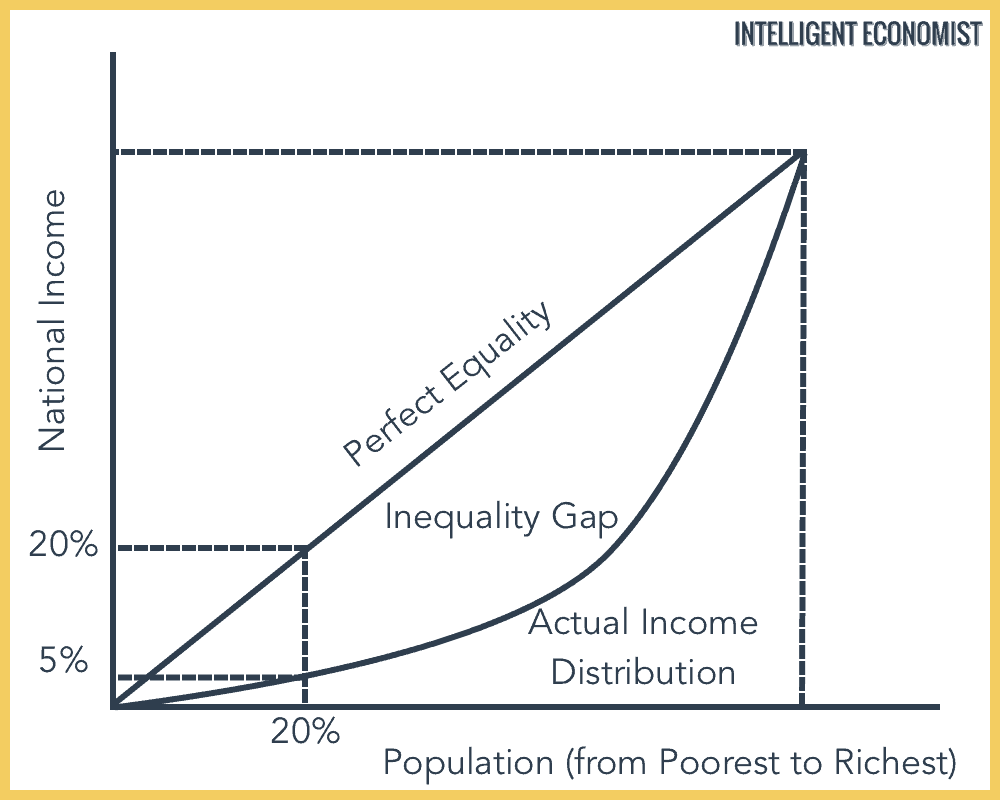
\includegraphics[width=0.5\textwidth]{03_Graphics/lorenz_curve}
\caption{Graph of Lorenz Curve \cite{CRYPTO:6}}
\end{center}
\end{figure}
A 45-degree line represents perfect wealth equality, so the Gini coefficient is essentially the ratio of the area that lies between the line of equality and the Lorenz curve. It is defined as one-half of the relative mean absolute difference: 
\begin{equation} 
G = \frac{\sum_{i=1}^{N}\sum_{j=1}^{N}\left | x_{i} - x_{j}\right |}{2 N^{2} \overline{x}} 
\end{equation}
where $x_{i}$ is the total wealth of person $i$ and $\overline{x}$ is the mean wealth across the population. Through the Gini coefficient, we can gain a significant understanding of the distribution of wealth as we simulate a Proof-of-Stake ecosystem.
